\documentclass{article}
% SPAIS / CoRL-format draft skeleton generated by smaj_v4.py. Put corl_2026.sty (from the template zip) next to this file;
% check the template's example.tex for the exact package options and the page limit.
\IfFileExists{corl_2026.sty}{\usepackage{corl_2026}}{\usepackage[margin=1in]{geometry}}
\usepackage{booktabs,graphicx,amsmath,hyperref}
% auto-generated by smaj_v4.py report
\newcommand{\EzeroSuccclean}{58/60}
\newcommand{\EzeroRMSTclean}{109}
\newcommand{\EzeroSucccovered}{10/60}
\newcommand{\EzeroRMSTcovered}{255}
\newcommand{\EzeroSuccscreened}{33/60}
\newcommand{\EzeroRMSTscreened}{193}
\newcommand{\EzeroSuccpainted}{44/60}
\newcommand{\EzeroRMSTpainted}{157}
\newcommand{\EzeroSuccrestoremlp}{59/60}
\newcommand{\EzeroRMSTrestoremlp}{108}
\newcommand{\EzeroSuccrestoreattr}{8/60}
\newcommand{\EzeroRMSTrestoreattr}{262}
\newcommand{\EzeroSuccrestorerandom}{8/60}
\newcommand{\EzeroRMSTrestorerandom}{260}
\newcommand{\EzeroSuccinjectattr}{60/60}
\newcommand{\EzeroRMSTinjectattr}{105}
\newcommand{\EzeroSuccrestoresel}{11/60}
\newcommand{\EzeroRMSTrestoresel}{254}
\newcommand{\EtwoSuccclean}{58/60}
\newcommand{\EtwoSucccovered}{10/60}
\newcommand{\EtwoSuccrestoremlp}{59/60}
\newcommand{\EtwoSuccrestoreattr}{8/60}
\newcommand{\EtwoSuccrestorerandom}{8/60}
\newcommand{\EtwoSuccinjectattr}{60/60}
\newcommand{\EtwoSuccrestoresel}{11/60}
\newcommand{\EtwoSuccrestoremlpLABD}{58/60}
\newcommand{\EtwoSuccrestoreseltopBAA}{10/60}
\newcommand{\EtwoSuccrestoreattrkDAA}{18/60}
\newcommand{\EtwoSuccrestoreattrkBAAA}{18/60}
\newcommand{\EtwoSuccrestorerandomkBAAA}{12/60}
\newcommand{\EtwoSuccrestorerandomkDAA}{8/60}
\newcommand{\EthreeAUROCsimple}{0.83}
\newcommand{\EthreeAUROCcoversel}{0.88}
\newcommand{\EthreeAUROCsimplecoversel}{0.89}
\newcommand{\EthreeAUROCcoverattr}{0.90}
\newcommand{\EthreeAUROCsimplecoverattr}{0.90}
\newcommand{\EthreeAUROCcoverseltopBAA}{0.88}
\newcommand{\EthreeAUROCsimplecoverseltopBAA}{0.89}
\newcommand{\EthreeAUROCcoverselall}{0.90}
\newcommand{\EthreeAUROCsimplecoverselall}{0.91}
\newcommand{\EthreeAUROCscreensel}{0.89}
\newcommand{\EthreeAUROCsimplescreensel}{0.91}
\newcommand{\EthreeAUROCvisibility}{0.91}
\newcommand{\EthreeAUROCsimplevisibility}{0.93}
\newcommand{\EthreeAUROCsaeall}{0.90}
\newcommand{\EthreeAUROCsimplesaeall}{0.91}
\newcommand{\EthreeAUROCdense}{0.89}
\newcommand{\EthreeAUROCsimpledense}{0.90}
\newcommand{\EfourGripAUROC}{1.00}
\newcommand{\EfourGripProprioAUROC}{1.00}

\title{Useful without being steerable: monitoring occlusion and gripper features in a VLA policy}
\begin{document}
\maketitle
\begin{abstract}
% One paragraph: problem (internal features for inspecting / monitoring / controlling robots), setting (pi0.5, LIBERO,
% rendered occluders), what was measured (task success, completion time, unwanted contact and lifting, early warning),
% the headline numbers from SUMMARY.md, and the take-away (monitoring value vs steering value).
\end{abstract}

\section{Introduction}
% Contextual hazards and runtime monitoring (Rethinking Safety for Generalist Robots); interpretable VLA features
% (Swann et al.; event-grounded SAEs); failure prediction from activations (action-expert probes). Our question:
% do features that fail as steering levers still help as monitors, measured by task-level and safety-relevant outcomes?

\section{Setup}
% Policy and hook site: PaliGemma language-prefix MLPs (18 layers), not the action expert. Transcoders (4096 features, k=64).
% Occluders: box (follows the target), screen (third-person camera only), static box (fixed, jittered), miss control.
\begin{figure}[t]\centering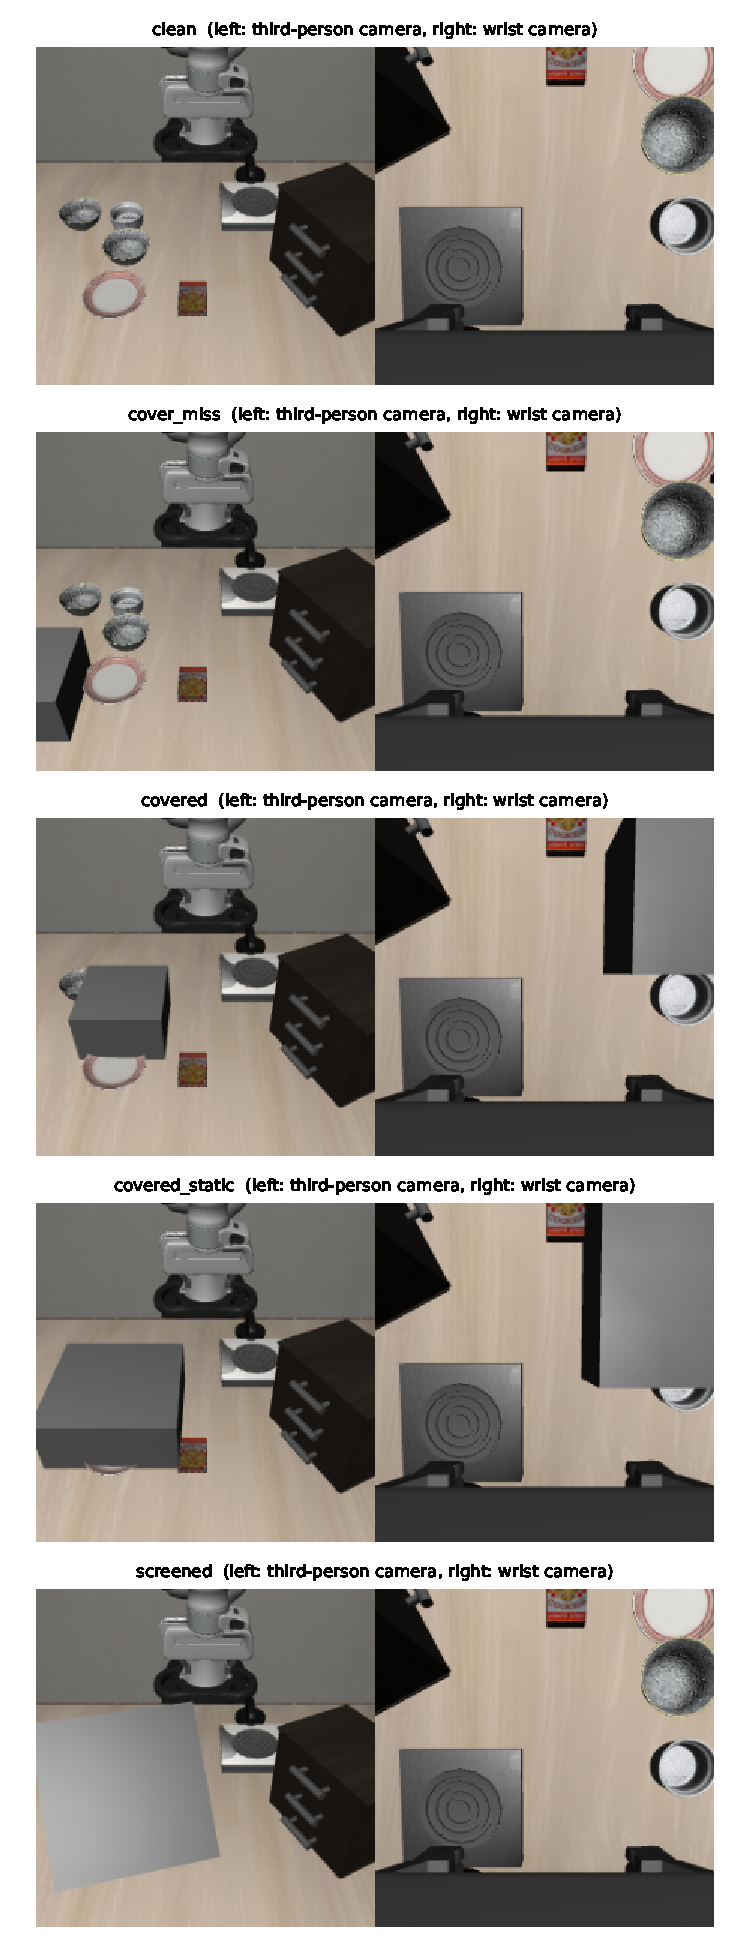
\includegraphics[width=0.8\linewidth]{figures/fig_conditions}
\caption{Conditions seen by the policy (third-person and wrist cameras).}\end{figure}

\section{Occlusion changes behaviour}
\begin{table}[t]
\centering\small
\caption{Closed-loop behaviour of the v3 conditions (5 tasks $\times$ 12 paired initial states). RMST: restricted mean completion time, failures counted at the step limit.}
\label{tab_E0_behaviour}
\begin{tabular}{l c c c c}
\toprule
condition & success & 95\% CI & RMST & distractor lifted \\
\midrule
clean & 58/60 &  [0.89, 0.99] & 109 & 0/60 \\
covered & 10/60 &  [0.09, 0.28] & 255 & 7/60 \\
screened & 33/60 &  [0.42, 0.67] & 193 & 0/60 \\
painted & 44/60 &  [0.61, 0.83] & 157 & 5/60 \\
restore mlp & 59/60 &  [0.91, 1.00] & 108 & 0/60 \\
restore attr & 8/60 &  [0.07, 0.24] & 262 & 6/60 \\
restore random & 8/60 &  [0.07, 0.24] & 260 & 7/60 \\
inject attr & 60/60 &  [0.94, 1.00] & 105 & 0/60 \\
restore sel & 11/60 &  [0.11, 0.30] & 254 & 7/60 \\
\bottomrule
\end{tabular}
\end{table}

\begin{figure}[t]\centering(figure fig_E0_success_by_step not available yet)
\caption{Cumulative success by control step; failed episodes never finish. Unlike mean completion time among successes,
this is not conditioned on success.}\end{figure}

\section{Features as monitors}
\begin{table}[t]
\centering\small
\caption{Failure prediction from information available after 48 control steps (out-of-fold, grouped by initial state). simple = proprioception, recent actions and task identity; visibility uses privileged segmentation.}
\label{tab_E3_monitor}
\begin{tabular}{l c c c}
\toprule
predictor & AUROC & AUPRC & recall@10\%FPR \\
\midrule
simple & 0.83 [0.79, 0.87] & 0.86 [0.81, 0.90] & 0.62 \\
cover sel & 0.88 [0.84, 0.91] & 0.87 [0.82, 0.92] & 0.71 \\
simple+cover sel & 0.89 [0.86, 0.92] & 0.89 [0.84, 0.94] & 0.75 \\
cover attr & 0.90 [0.86, 0.92] & 0.90 [0.86, 0.93] & 0.69 \\
simple+cover attr & 0.90 [0.87, 0.93] & 0.91 [0.88, 0.94] & 0.72 \\
cover sel top100 & 0.88 [0.85, 0.92] & 0.88 [0.84, 0.92] & 0.70 \\
simple+cover sel top100 & 0.89 [0.85, 0.92] & 0.90 [0.86, 0.93] & 0.73 \\
cover sel all & 0.90 [0.87, 0.93] & 0.89 [0.85, 0.93] & 0.77 \\
simple+cover sel all & 0.91 [0.88, 0.94] & 0.91 [0.88, 0.95] & 0.81 \\
screen sel & 0.89 [0.86, 0.92] & 0.91 [0.87, 0.93] & 0.73 \\
simple+screen sel & 0.91 [0.88, 0.93] & 0.92 [0.89, 0.95] & 0.77 \\
visibility & 0.91 [0.88, 0.94] & 0.90 [0.86, 0.93] & 0.76 \\
simple+visibility & 0.93 [0.91, 0.95] & 0.94 [0.91, 0.96] & 0.80 \\
sae all & 0.90 [0.88, 0.93] & 0.91 [0.88, 0.94] & 0.77 \\
simple+sae all & 0.91 [0.88, 0.94] & 0.92 [0.89, 0.95] & 0.80 \\
dense & 0.89 [0.86, 0.92] & 0.91 [0.87, 0.94] & 0.69 \\
simple+dense & 0.90 [0.87, 0.93] & 0.91 [0.87, 0.94] & 0.76 \\
\bottomrule
\end{tabular}
\end{table}

\begin{figure}[t]\centering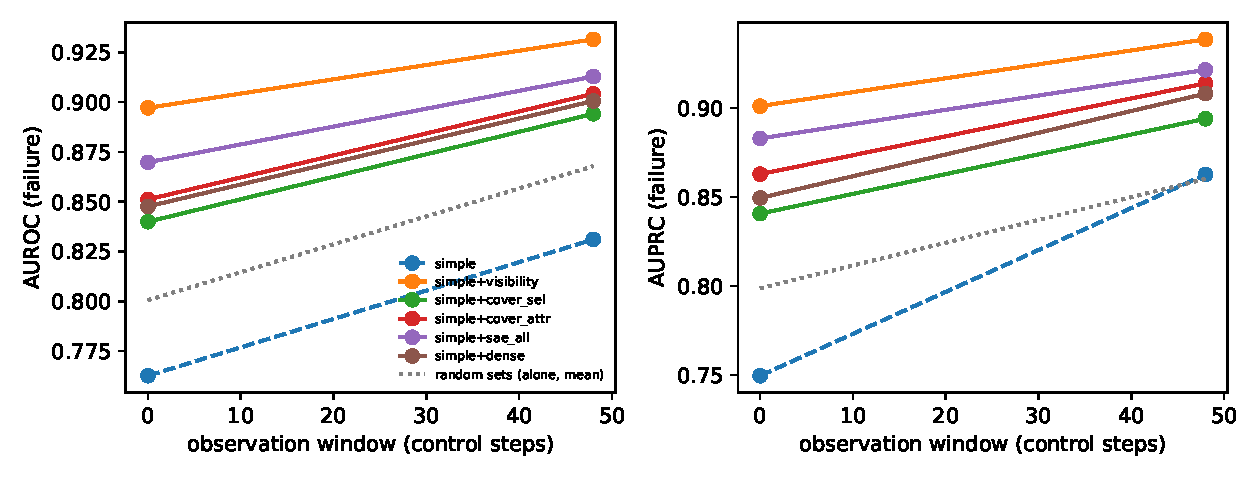
\includegraphics[width=0.9\linewidth]{figures/fig_E3_monitor_windows}
\caption{Failure prediction by observation window.}\end{figure}
\begin{figure}[t]\centering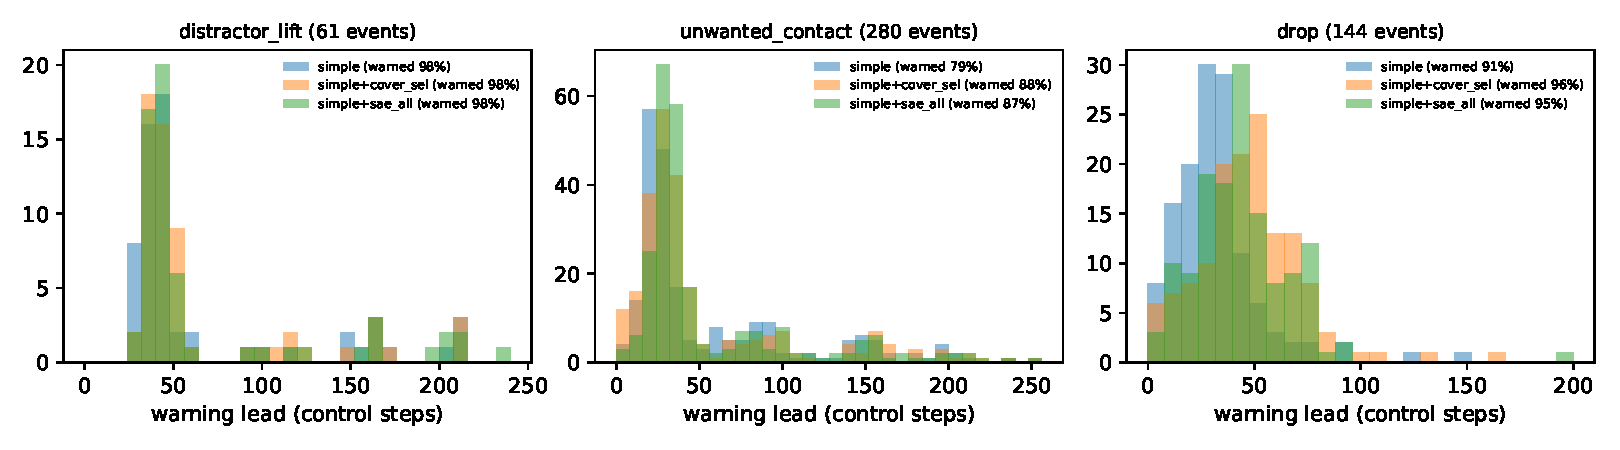
\includegraphics[width=0.9\linewidth]{figures/fig_E3_lead_time}
\caption{Warning lead time before unwanted events at a fixed 10\% false-alarm rate.}\end{figure}

\section{Features as levers}
\begin{figure}[t]\centering(figure fig_E4_grip_trace not available yet)
\caption{Gripper-feature score aligned to the close command (discovery and held-out episodes).}\end{figure}
\begin{table}[t]
\centering\small
\caption{Paired effects of steering, prompting and action scaling (same initial states; task-clustered CIs).}
\label{tab_E5_steer}
\begin{tabular}{l c c c}
\toprule
comparison & $\Delta$ success & $\Delta$ speed & $\Delta$ first close \\
\midrule
prompt slow vs base & -0.020 [-0.120, 0.060] & -0.006 [-0.011, -0.000] & 0.120 [-0.060, 0.300] \\
act scale vs base & -0.760 [-0.980, -0.520] & -0.097 [-0.106, -0.088] & 4.560 [0.000, 10.640] \\
speed ablate vs base & 0.000 [-0.060, 0.060] & -0.001 [-0.004, 0.003] & 0.040 [0.000, 0.080] \\
speed boost vs base & 0.040 [0.000, 0.080] & -0.000 [-0.007, 0.004] & -0.060 [-0.260, 0.140] \\
speed random vs base & 0.000 [0.000, 0.000] & -0.002 [-0.004, -0.000] & -0.020 [-0.060, 0.000] \\
grip ablate vs base & 0.000 [-0.060, 0.060] & -0.003 [-0.006, 0.000] & 0.000 [0.000, 0.000] \\
grip boost vs base & 0.000 [-0.060, 0.060] & -0.004 [-0.008, -0.000] & -0.240 [-0.620, 0.180] \\
grip random vs base & 0.020 [0.000, 0.060] & -0.002 [-0.008, 0.003] & 0.760 [0.160, 1.660] \\
covered prompt slow vs covered & 0.020 [-0.040, 0.080] & -0.001 [-0.007, 0.004] & 0.420 [0.120, 0.720] \\
covered act scale vs covered & -0.120 [-0.220, -0.020] & -0.036 [-0.053, -0.020] & 9.940 [1.940, 17.940] \\
speed ablate vs speed random & 0.000 [-0.060, 0.060] & 0.001 [-0.003, 0.005] & 0.060 [0.020, 0.100] \\
grip boost vs grip random & -0.020 [-0.080, 0.040] & -0.002 [-0.010, 0.006] & -1.000 [-1.560, -0.540] \\
speed ablate vs prompt slow & 0.020 [-0.040, 0.080] & 0.005 [0.000, 0.010] & -0.080 [-0.220, 0.080] \\
speed ablate vs act scale & 0.760 [0.540, 0.940] & 0.096 [0.089, 0.105] & -4.520 [-10.560, 0.040] \\
speed boost vs prompt slow & 0.060 [0.000, 0.140] & 0.006 [0.000, 0.012] & -0.180 [-0.360, 0.060] \\
covered prompt slow vs covered act scale & 0.140 [0.040, 0.240] & 0.036 [0.023, 0.052] & -9.520 [-17.600, -1.440] \\
\bottomrule
\end{tabular}
\end{table}

\begin{table}[t]
\centering\small
\caption{Restoring clean values under the box occluder at every inference step. Recovered fraction = (restored $-$ occluded)/(clean $-$ occluded) success, task-clustered bootstrap CI.}
\label{tab_E2_controls}
\begin{tabular}{l c c c}
\toprule
condition & success & 95\% CI & recovered fraction \\
\midrule
clean & 58/60 &  [0.89, 0.99] & -- \\
covered & 10/60 &  [0.09, 0.28] & -- \\
restore mlp & 59/60 &  [0.91, 1.00] & 1.02 [0.95, 1.16] \\
restore attr & 8/60 &  [0.07, 0.24] & -0.04 [-0.24, 0.06] \\
restore random & 8/60 &  [0.07, 0.24] & -0.04 [-0.15, 0.04] \\
inject attr & 60/60 &  [0.94, 1.00] & -- \\
restore sel & 11/60 &  [0.11, 0.30] & 0.02 [0.00, 0.06] \\
restore mlp L0 13 & 58/60 &  [0.89, 0.99] & 1.00 [0.93, 1.14] \\
restore sel top100 & 10/60 &  [0.09, 0.28] & 0.00 [0.00, 0.00] \\
restore attr k300 & 18/60 &  [0.20, 0.43] & 0.17 [0.04, 0.36] \\
restore attr k1000 & 18/60 &  [0.20, 0.43] & 0.17 [-0.14, 0.37] \\
restore random k1000 & 12/60 &  [0.12, 0.32] & 0.04 [-0.05, 0.15] \\
restore random k300 & 8/60 &  [0.07, 0.24] & -0.04 [-0.15, 0.04] \\
\bottomrule
\end{tabular}
\end{table}

\begin{figure}[t]\centering(figure fig_E2_dose not available yet)
\caption{Restoring clean feature values under the box occluder: attribution top-K, matched random sets and full-MLP bounds.}\end{figure}

\section{Limitations}
% One policy and suite for the closed loop; simulation; render-only occluders; dictionary fidelity (E6);
% control steps not seconds unless the 20 Hz control rate is confirmed; privileged clean renders for restoration.

\bibliographystyle{plainnat}
\bibliography{references_v4}
\end{document}
